\begin{figure*}
\centering
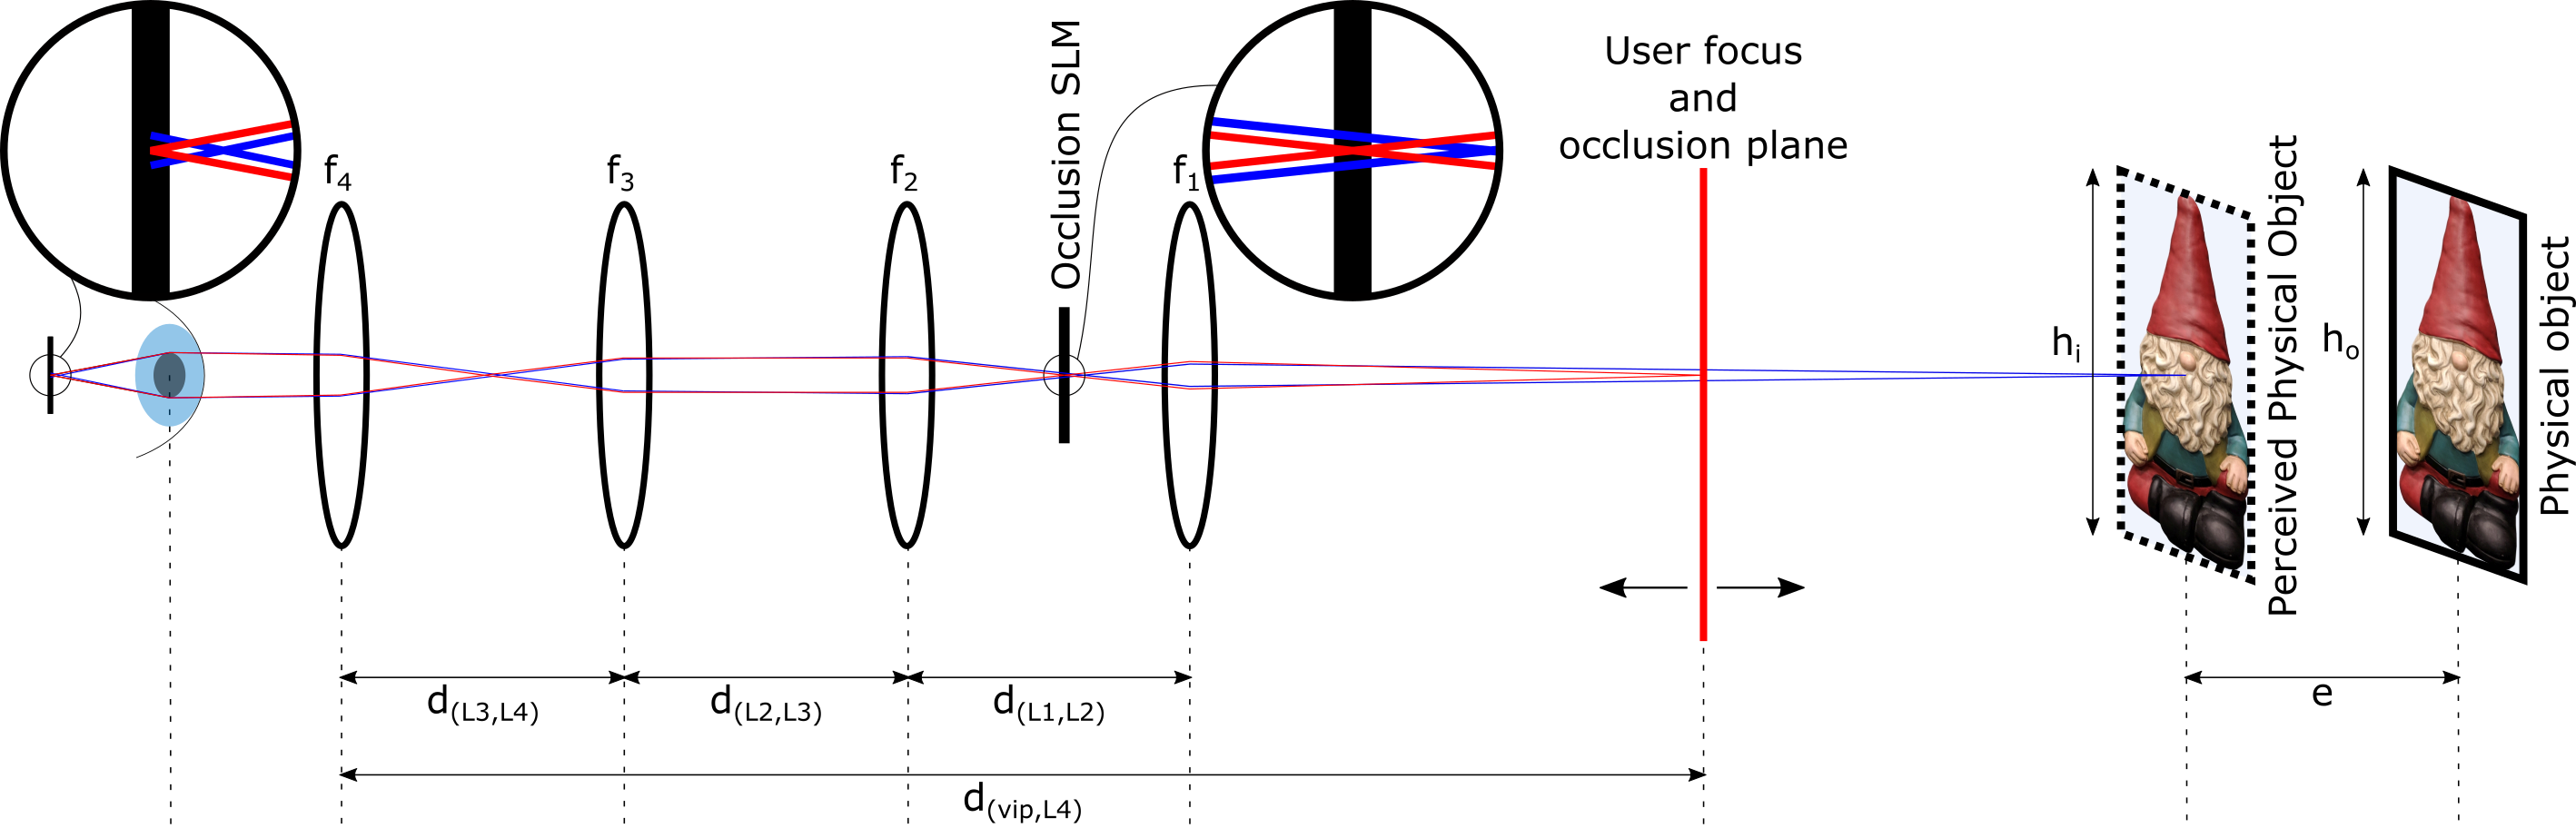
\includegraphics[width=0.89\textwidth]{images/varifocal_occlusion/unfolded}
%\fbox{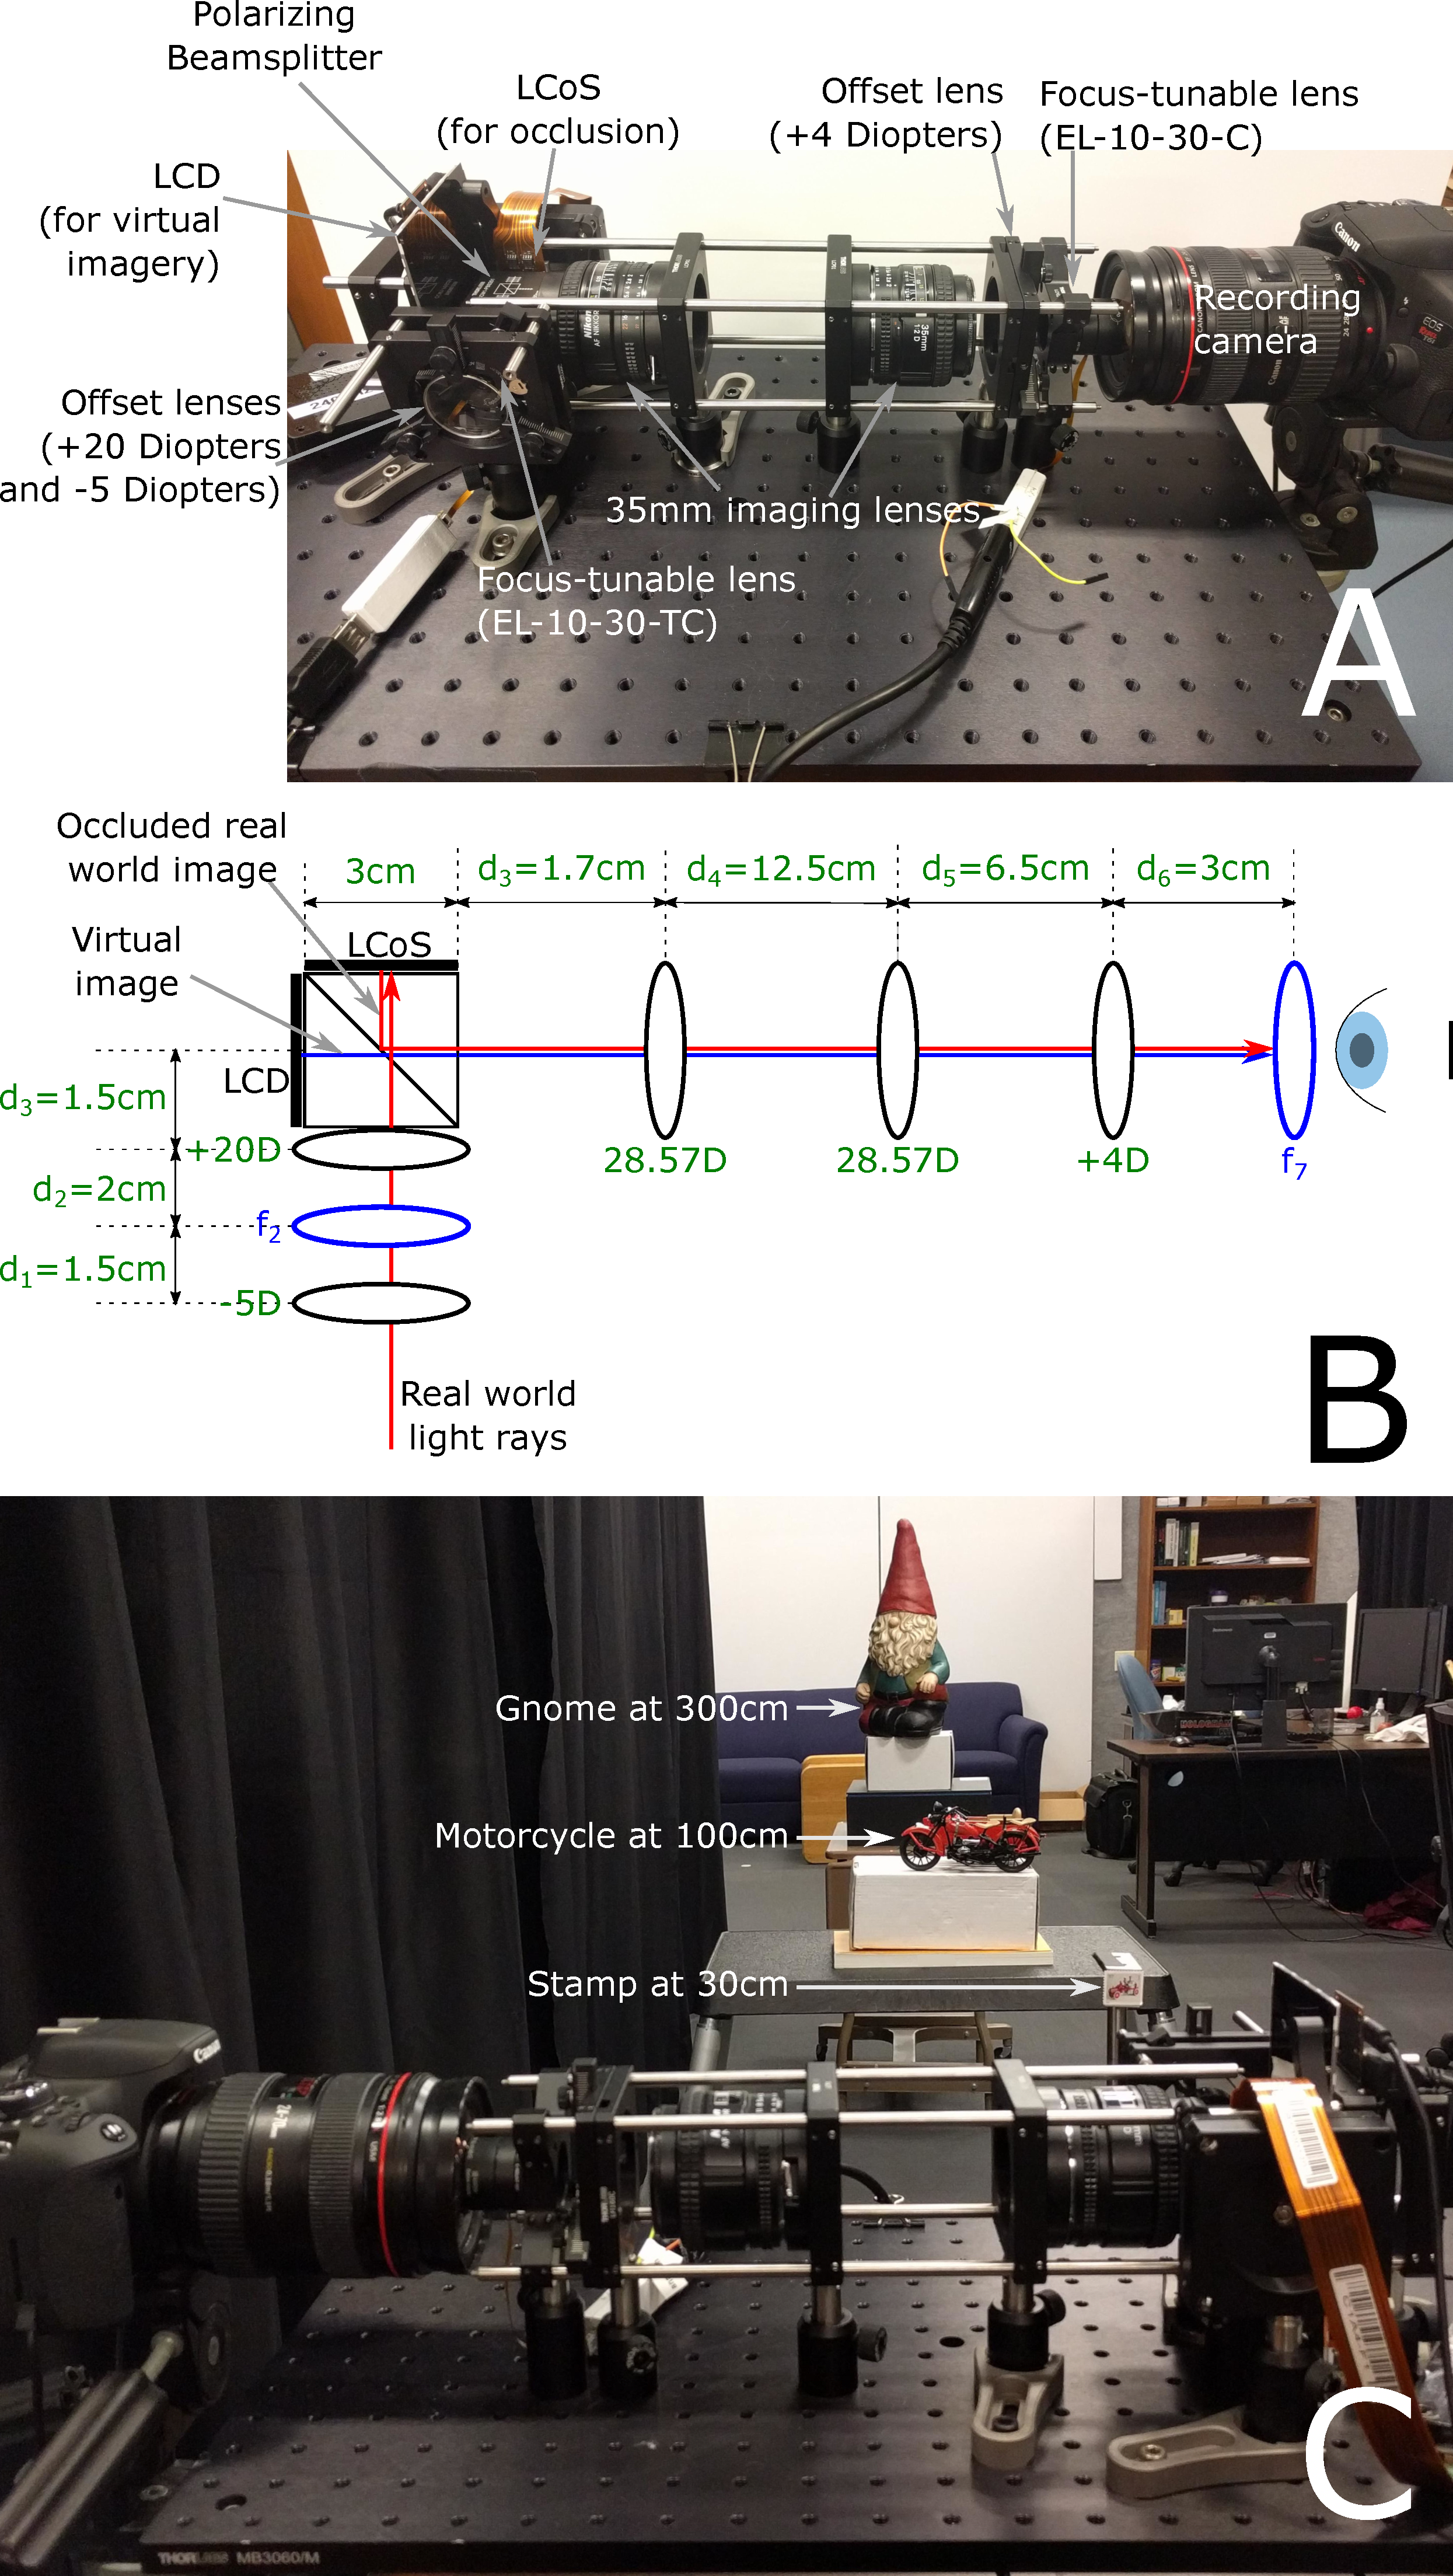
\includegraphics[width=0.46\textwidth]{images/prototype}}
\caption[Varifocal-Occlusion: unfolded optics]{Illustration of the unfolded optical path of a 4-lens system for image-forming occlusion-capable AR displays. With a varifocal display, the distance of virtual image and occlusion mask matches the user's focus distance, indicated by the thick vertical red line. Red and blue lines going from points in the scene through the optics onto the retina indicate ray diagrams for the image formation of the virtual/occlusion image and for physical objects, respectively. Enlarged inset at the occlusion SLM shows that the physical world at the user's focus plane is brought into focus at the SLM where portions of the real world can be occluded. Enlarged inset at the retina shows that the same rays (red) that are in-focus at the occlusion SLM are also in-focus at the retina -- this property is utilized to also depict a perceptually correct occlusion mask for out-of-focus virtual objects by applying a computational blur. Finally, the image of real-world objects seen through the display should ideally have the same magnification and distances from the eye as compared to seeing the real world without the display, i.e. $\frac{h_i}{h_o}=1$ and $e=0$. In our implementation, we are able to match the magnification, but not the distance.}
\label{fig:varifocal_occlusion:unfolded}
\end{figure*}

Our goal is to design a varifocal occlusion-capable OST AR display that satisfies several key requirements. These include 
%
\begin{enumerate}
    \item The virtual image of the occlusion SLM, i.e., the occlusion mask, and the digital image should be optically placed together in the scene and their distance be dynamically adjustable.
    \item The lateral and longitudinal magnification of the physical scene seen through the display should be equal to one, such that the experience is similar to viewing the scene without any optical elements.
    \item No mechanical motion should be introduced to any component (lenses, SLM, etc.) to adjust the distance of its virtual image. Instead, the virtual image should be moved by changing the focal powers of the employed lenses.
\end{enumerate}
%

In the following, we first provide an overview of the optical design we consider, introduce a ray-transfer matrix analysis of prior work on fixed-focus occlusion-capable AR displays (see Sec.~\ref{sec:varifocal_occlusion:related:fixedfocusOcc}), and finally introduce our focus-tunable varifocal occlusion approach.

\paragraph{\textbf{Overview of the optical design}}
We consider an optical design composed of four lenses (see Fig.~\ref{fig:varifocal_occlusion:unfolded}), whose respective functions are: The first lens brings the real world at a particular depth into focus at the SLM. This image is always flipped, similar to how the image of the real world that is formed on our retina inside our eyes is always flipped. The next two lenses re-invert the in-focus image at the SLM, similar to a 4f system. The last lens finally places the image back into the appropriate depth for comfortable viewing. Let us denote these lenses by $L_1,L_2,L_3,L_4$ (see Fig.~\ref{fig:varifocal_occlusion:unfolded}).

The occlusion SLM can be placed in either of the image planes of the optical system. One is between $L_1$ and $L_2$, and the other is between $L_3$ and $L_4$. We place the occlusion SLM between $L_1$ and $L_2$ because it simplifies Eq.~\eqref{eq:closed_form_f_1}. The digital image SLM can also be placed in any of the image planes of the optical system. We choose to place it between $L_1$ and $L_2$ because in this case, we can treat both the occlusion SLM and the virtual SLM to be optically equivalent and derive just one set of conditions for both of them.

%%%%%%%%%%%%%%%%%%%%%%%%%%%%%%%%%%%%%%%%%%%%%%%%%%%%%%%%%%%%%%%%%%%%%%%%%%%%%%%%%%%%%%%%%%%%%%%%%%
\subsection{Modeling Fixed-focus Occlusion Masks}
\label{sec:optical_design_fixed_focus}

%In this subsection, we discuss previous approaches to display an occlusion mask at a fixed depth. Such systems satisfy the first three requirements listed earlier. We restrict the discussion of previous works to the image-forming occlusion type. 

%\kishore{Move to related work}
%Kiyokawa et al. \cite{Kiyokawa2003} derive optical design parameters that satisfy unit magnification for all real-world object distances and propose an interesting geometric configuration of the optical components that make the offset between the real-world objects and images equal to zero.
%Cakmakci et al. \cite{Cakmakci2004} propose a compact optical design that satisfies the magnification requirements. 
%Cakmakci et al.'s \cite{Cakmakci2004} design does not guarantee that the offset between the real viewpoint and the virtual viewpoint should be zero; however, the offset is small (5 cm). 
%The design approach in these papers was primarily based on algebraic analysis of the Gaussian form of the thin lens equation to guarantee that the magnification is one, and coming up with an interesting folded optics design to ensure that the real viewpoint and virtual viewpoint are coincident, if possible. 

%Other previous papers propose a more general approach based on ray-transfer matrix analysis, summarized below.

%\subsubsection{Ray-transfer matrix}

The light transport through optical components can be modeled using ray-transfer matrices. In this approach, a light ray is represented by a column vector composed of lateral distance ($x$) and angle of propagation ($\theta$) with respect to the optical axis. 
The propagation of paraxial light rays through an optical component is modeled as the multiplication of the ray vector with a $2 \times 2$ ray-transfer matrix. Ray-transfer matrices are known for standard optical components, e.g. let us denote the ray-transfer matrix for a lens with focal length $f$ by $\mathbf{M}$ and the ray-transfer matrix for free-space propagation with a distance $d$ by $\mathbf{S}$. Then, $\mathbf{M}$ and $\mathbf{S}$ are given by:

%
\begin{equation}
\mathbf{M} = 
\begin{bmatrix}
1 & 0 \\
-\frac{1}{f} & 1 
\end{bmatrix},
\quad \quad
\mathbf{S} = 
\begin{bmatrix}
1 & d \\
0 & 1 
\end{bmatrix}.
\end{equation}
%
The composite ray transfer matrix that models the propagation of light rays through a series of optical components is simply the multiplication of the various individual ray transfer matrices of each optical component. 

For our optical design (Fig.~\ref{fig:varifocal_occlusion:unfolded}), the composite ray transfer matrix is represented as:
%
\begin{equation}
\mathbf{T} = \mathbf{M}_4 \mathbf{S}_{(L_3,L_4)} \mathbf{M}_3 \mathbf{S}_{(L_2,L_3)} \mathbf{M}_2 \mathbf{S}_{(L_1,L_2)} \mathbf{M}_1,
\label{eq:static_general}
\end{equation}
%
where $\mathbf{M}_i$ is the ray-transfer matrix describing $L_i$ and $\mathbf{S}_{(L_i,L_j)}$ describes the free-space propagation between lenses $L_i$ and $L_j$.

The above linear system of equations is composed of four equations and seven unknowns (four unknown focal lengths and three unknown distances). This is an ill-posed inverse problem. Instead of attempting to solve it directly, previous works relied on symmetry constraints, such that $f_1 = f_4$, $f_2 = f_3$, and $d_{(L_1,L_2)} = d_{(L_3,L_4)}$.

%which makes the composite ray transfer matrix:
%
%\begin{equation}
%T = M_1 S_{(1,2)} M_2 S_{(2,3)} M_2 S_{(1,2)} M_1.
%\label{eq:static_symmetric}
%\end{equation}
%
%This system of linear equations has four unknowns and is solvable analytically.

Previous works have explored mainly two choices for the composite ray transfer matrix.

{\bf Shifted Perspective. $\,\,$}
In this configuration, the virtual viewpoint is shifted to the front of the optical system. In other words, the first lens and the last lens form conjugate aperture planes. Another way to think of it is that the light field entering the optical system and the light field exiting the optical system are equivalent. Mathematically, this condition represents $\mathbf{T} = \mathbf{I}$, where $\mathbf{I}$ is the $2 \times 2$ identity matrix. Some of the earlier prototypes of \citet{Kiyokawa2000,Kiyokawa2001} and \citet{Cakmakci2004} had a shifted perspective. 

{\bf Correct Perspective. $\,\,$}
In this configuration, a user looking through the optical system should see the exact same image of a physical scene behind it as if the optical system was absent. There is no shift in the viewpoint. \citet{Kiyokawa2003} proposed a folded optics design for achieving correct perspective. This condition was analyzed formally with ray-transfer matrix equations for the first time in the context of optical cloaking~\cite{Choi2015} and later applied to the problem of occlusion in AR displays~\cite{Howlett2017}. Mathematically, this is represented via the ray-transfer matrix $\mathbf{T} = \mathbf{S}_{(L_1,L_4)}$.

%\paragraph{Choosing between the two constraints}
While an OST AR display should ideally be made to satisfy the correct perspective constraint, the disadvantage in doing so is that the field of view of the optical system is much smaller, being at most equal to the field of view seen through the first lens' aperture from a viewing distance of the length of the optical system. This limitation is exacerbated in our implementation by the small aperture (1 cm) of our focus-tunable lenses. For this reason, we design and implement an optical system that satisfies the shifted-perspective constraint. 

%\subsubsection{Previous approach applied to varifocal occlusion}
%The optical design solution which was calculated using ray-transfer matrix approach in the previous works will extend to a varifocal occlusion display trivially, but will require all the fixed-focal length lenses to be replaced by focus-tunable lenses and will require that the lenses be movable dynamically. Mathematically, having all lenses and distances as dynamic parameters, with the symmetry constraints of $f_1^{(t)} = f_4^{(t)}$, $f_2^{(t)} = f_3^{(t)}$, and $d_{(L_1,L_2)}^{(t)} = d_{(L_3,L_4)}^{(t)}$, the ray-transfer matrix would be:
%\begin{equation}
%    T = M_1^{(t)} S_{(1,2)}^{(t)} M_2^{(t)} S_{(2,3)}^{(t)} M_2^{(t)} S_{(1,2)}^{(t)} M_1^{(t)},
%\end{equation}
%where we denote dynamic parameters with the superscript $^{(t)}$.
%This would result in an overly complicated system. Below, we discuss our approach.


%%%%%%%%%%%%%%%%%%%%%%%%%%%%%%%%%%%%%%%%%%%%%%%%%%%%%%%%%%%%%%%%%%%%%%%%%%%%%%%%%%%%%%%%%%%%%%%%%%
\subsection{Modeling Varifocal Occlusion Masks}
\label{sec:optical_design:varifocal_occlusion_mask}

Consider the general system of linear equations for image-forming occlusion optical designs (Eq.~\eqref{eq:static_general}). Recall that solving this is not possible by simply analyzing the ray-transfer matrix equations because there are more unknowns than equations. Our approach is to apply an optimization approach to this problem. Gaining some insights from the optimization approach, we then revisit the ray-transfer matrices approach to derive closed-form solutions.

Both our approaches aim to satisfy these requirements:
\begin{enumerate}
   \item  
    the virtual image should be placed at a desired (but movable) distance.
    \item 
    the magnification of the see-through image of the real-world should be unity irrespective of the virtual image plane distance. 
\end{enumerate}

\subsubsection{Optimization approach}
\label{sec:optical_design_optimization}
The optimization approach needs to calculate the set of focal lengths that minimize the error in the magnification of the see-through view and the error in the virtual/occlusion image plane's depth.

To do this, we define an image formation model for OST occlusion-capable displays, a cost function for the errors, and apply known methods to minimize the error iteratively. We start off by assuming that all lenses are focus-tunable lenses.

\paragraph{\textbf{Image Formation}}
The image formation for the virtual and real-world is modeled by successive application of the Gaussian thin lens equations:

\begin{equation}
i = \frac{o f}{o - f},
\label{eq:gaussian_thin_lens_equation}
\end{equation}
where $i$ is the image distance, $o$ is the object distance, and $f$ is the focal length of the lens.

For an optical system composed of multiple lenses, the object of the subsequent lens ($L_{j+1}$) is the image of the previous lens ($L_{j}$). So, the object distance for $L_{j+1}$ is: $o_{j+1} = d_{(L_j, L_{j+1})} - i_j$.

\paragraph{\textbf{Occlusion and Virtual Image Formation}}
For the occlusion and virtual image, the objects are the occlusion and virtual SLMs which are optically placed together by design. Only the lenses between these SLMs and the eye ($L_2,L_3,L_4$) contribute to the virtual/occlusion image formation. So, the object distance ($d_{(\text{SLM},L_2)}$) is propagated through lenses $L_2$, $L_3$, and $L_4$, to obtain the distance to the perceived occlusion/virtual image plane from lens 4 ($d_{(\text{vip},L_4)}$). Let us denote this image formation function by:
\begin{equation}
[d_{(\text{vip},L_4)}] = I_V(f_2, f_3, f_4, d_{(\text{SLM}, L_2)}, d_{(L_2,L_3)}, d_{(L_3,L_4)}),
\label{eq:optimization_virtual_image_formation}
\end{equation}
where $I_V$ is composed of the successive application of Eq.~\eqref{eq:gaussian_thin_lens_equation}, beginning with
\begin{equation}
i_2 = \frac{d_{(\text{SLM},L_2)} f_2}{d_{(\text{SLM},L_2)}-f_2},
\quad \quad
o_{3} = d_{(L_2,L_3)} - i_2,
\end{equation}
and ending with:
\begin{equation}
d_{(\text{vip},L_4)} = \frac{o_4 f_4}{o_4 - f_4}.
\end{equation}

\paragraph{\textbf{See-Through Image Formation}}
For the real-world, we first discretize the real-world into $N$ real-world depth planes, where the number $N$ is chosen such that the system samples the real-world denser than the human eye's depth-of-field which has been measured to be $0.3$ diopters~\cite{Campbell1957,Watt2005}. So, for a display whose nearest and farthest depth planes are at $D_{(R_{\text{near}}, L_1)}$ diopters and $D_{(R_{\text{far}}, L_1)}$ diopters respectively, the minimum number of discretized real-world depth planes should be:

\begin{equation}
N > \frac{D_{(R_{\text{near}},L_1)} - D_{(R_{\text{far}},L_1)}}{0.3}.
\label{eq:optimization:number_of_planes}
\end{equation}

Each real-world depth ($d_{(R_j,L_1)}$) is propagated through lenses $L_1,L_2,L_3,L_4$ from which we get the see-through image depth from $L_4$ ($d_{(V_j,L_4)}$):
\begin{align}
&[d_{(V_1,L_4)}, d_{(V_2,L_4)},...,d_{(V_N,L_4)}] = \nonumber\\
&I_R(f_1, f_2, f_3, f_4, d_{(L_1,L_2)}, d_{(L_2,L_3)}, d_{(L_3,L_4)}, d_{(R_1,L_1)},d_{(R_2,L_1)},...,d_{(R_N,L_1)}),
\label{eq:optimization_real_image_formation}
\end{align}
where $I_R$ is a successive application of Eq.~\eqref{eq:gaussian_thin_lens_equation} for each discretized real-world depth plane beginning with:
\begin{equation}
i_1 = \frac{d_{(R_j,L_1)} f_1}{d_{(R_j,L_1)}-f_1},
\quad \quad
o_{2} = d_{(L_1,L_2)} - i_1,
\end{equation}
and ending with:
\begin{equation}
d_{(V_j,L_4)} = \frac{o_4 f_4}{o_4 - f_4}.
\end{equation}

\paragraph{\textbf{Error function}}
The error associated with the occlusion/virtual image is the difference between desired occlusion/virtual image plane depth ($d_{in}$) and actual occlusion/virtual image plane depth ($d_{(\text{vip},L_4)}$) calculated as: $d_{in} - d_{(\text{vip},L_4)}$.

The error associated with the magnification of the physical scene is the difference between one and the magnification of the see-through image, where magnification is calculated as $m = -\frac{\text{image distance}}{\text{object distance}}$. However, in calculating the magnification, we need to be careful about what we consider as the object distance: Recall that in the see-through image formation function (Eq.~\eqref{eq:optimization_real_image_formation}), we've defined the real-world object distances with respect to the first lens ($d_{(R_j, L_1)}$), whereas the final image distance is calculated with respect to the last lens ($d_{(V_j, L_4)}$). This discrepancy is alright when the optical system is designed to satisfy the shifted-perspective constraint. However, for the correct-perspective constraint, the object distance should be modified to $d_{(R_j,L_1)}+d_{(L_1,L_4)}$. For our display, where the correct object distance is $d_{(R_j,L_1)}$ and the magnification is given by $m_j=-\frac{d_{(V_j,L_4)}}{d_{(R_j,L_1)}}$

The combined error vector is given below:
\begin{equation}
    E = 
    \begin{bmatrix} 
    d_{\text{in}} - d_{(\text{vip},L_4)}\\ 
    1 - m_1\\ 
    1 - m_2\\ 
    ...\\ 
    1 - m_N\\ 
    \end{bmatrix}.
    \label{eq:optimization_error}
\end{equation}

The optimization problem is to find a set of focal lengths ($f_1,f_2,f_3,f_4$) that minimize the above error:
\begin{equation}
\argmin_{f_1,f_2,f_3,f_4} ||E||^2.
\end{equation}

Our implementation of this indicates that the set of focal lengths that minimizes the above error function always has a fixed $f_2$ and $f_3$. 

Unfortunately, the execution time of this optimization is not real-time. We could calculate the dynamic values of $f_1$ and $f_4$ for different occlusion mask distances and use the calculated values in a look-up table to get real-time performance. Alternatively, we could use the new information that a fixed $f_2$ and $f_3$ can satisfy all the requirements to calculate closed-form solutions, as discussed below.

\subsubsection{Closed-form solutions}
\label{sec:optical_design_closed_form}

Consider the same 4-lens optical design for a varifocal occlusion-capable display composed of the following parameters: $f_1^{(t)}, f_2, f_3, f_4^{(t)}, d_{(L_1,L_2)}, d_{(L_2,L_3)}, d_{(L_3,L_4)}, d_{(\text{SLM},L_1)}$, where the superscript $\cdot ^{(t)}$ indicates a dynamically changing parameter. 


Using the Gaussian thin lens equation (Eq.~\eqref{eq:gaussian_thin_lens_equation}), $f_1^{(t)}$ is calculated based on the desired virtual image plane distance ($d_{(\text{vip},L_1)}^{(t)}$) and the distance between $L_1$ and the occluding SLM ($d_{(\text{SLM},L_1)}$):
\begin{equation}
    f_1^{(t)} = \frac{d_{(\text{vip},L_1)}^{(t)} d_{(\text{SLM},L_1)} }{d_{(\text{vip},L_1)}^{(t)} + d_{(\text{SLM},L_1)} }.
    \label{eq:closed_form_f_1}
\end{equation}

Solving for the rest of the parameters needs an analysis of the ray-transfer matrix equation. To satisfy the shifted-perspective condition, the ray-transfer matrix needs to satisfy:
\begin{equation}
    \mathbf{I} = \mathbf{M}_4^{(t)} \mathbf{S}_{(L_3,L_4)} \mathbf{M}_3 \mathbf{S}_{(L_2,L_3)} \mathbf{M}_2 \mathbf{S}_{(L_1,L_2)} \mathbf{M}_1^{(t)}.
    \label{eq:II_eq_TA}
\end{equation}
Finding optical parameter values that satisfy the above equation automatically ensures that the requirements listed in the beginning of Sec.~\ref{sec:optical_design:varifocal_occlusion_mask} will be satisfied. Since we have learned from our optimization experiments that solutions exists where $L_2$ and $L_3$ are fixed-focal length lenses, we solve Eq.~\eqref{eq:II_eq_TA} for $\mathbf{M}_4^{(t)}$ and analyze the conditions that ensure that the constants of matrix $\mathbf{M}_4^{(t)}$ (i.e., the ones and zero of $\mathbf{M}_4^{(t)}$) are their appropriate values: 

\begin{equation}
\mathbf{M}_4^{(t)} \overset{a}{=} 
\begin{bmatrix}
\frac{1 + BC}{\frac{C}{f_1^{(t)}} + A} & C \\
B & \frac{C}{f_1^{(t)}} + A
\end{bmatrix}
\overset{b}{=}
\begin{bmatrix}
1 & 0 \\
-\frac{1}{f_4^{(t)}} & 1 
\end{bmatrix},
\label{eq:closed_form_I}
\end{equation}
where $\overset{a}{=}$ is obtained by solving Eq.~\eqref{eq:II_eq_TA} for $\mathbf{M}_4^{(t)}$ and $\overset{b}{=}$  is obtained because $\mathbf{M}_4^{(t)}$ should have the ray-trasfer matrix for a lens, and where $A$, $B$, $C$ are the following:
% \begin{flalign}
% &A = 1 - \frac{d_{(L_3,L_4)} + d_{(L_2,L_3)} \left(1 - \frac{d_{(L_3,L_4)}}{f_{3}}\right)}{f_{2}} - \frac{d_{(L_3,L_4)}}{f_{3}}, \label{eq:shifted_perspective_A} \\ 
% &B = \frac{1 - \frac{d_{(L_2,L_3)}}{f_{3}} - d_{(L_1,L_2)} \left(\frac{1 - \frac{d_{(L_2,L_3)}}{f_{3}}}{f_{2}} + \frac{1}{f_{3}}\right)}{f_1^{(t)}} + \frac{1 - \frac{d_{(L_2,L_3)}}{f_{3}}}{f_{2}} + \frac{1}{f_{3}}, \label{eq:shifted_perspective_B} \\
% &C = d_{(L_2,L_3)} \left(1 - \frac{d_{(L_3,L_4)}}{f_{3}}\right) + d_{(L_3,L_4)} + d_{(L_1,L_2)}A. \label{eq:shifted_perspective_C}
% \end{flalign}

\begin{equation}
    A = 1 - \frac{d_{(L_3,L_4)} + d_{(L_2,L_3)} \left(1 - \frac{d_{(L_3,L_4)}}{f_{3}}\right)}{f_{2}} - \frac{d_{(L_3,L_4)}}{f_{3}}, \label{eq:shifted_perspective_A}
\end{equation}

\begin{equation}
    B = \frac{1 - \frac{d_{(L_2,L_3)}}{f_{3}} - d_{(L_1,L_2)} \left(\frac{1 - \frac{d_{(L_2,L_3)}}{f_{3}}}{f_{2}} + \frac{1}{f_{3}}\right)}{f_1^{(t)}} + \frac{1 - \frac{d_{(L_2,L_3)}}{f_{3}}}{f_{2}} + \frac{1}{f_{3}},
    \label{eq:shifted_perspective_B}
\end{equation}

\begin{equation}
    C = d_{(L_2,L_3)} \left(1 - \frac{d_{(L_3,L_4)}}{f_{3}}\right) + d_{(L_3,L_4)} + d_{(L_1,L_2)}A.
    \label{eq:shifted_perspective_C}
\end{equation}

From Eq.~\eqref{eq:closed_form_I}, we can infer that $C=0$, and thereby, we can derive that $A=1$ by substituting $C=0$ in:
\begin{equation}
    1 = \frac{C}{f_1^{(t)}} + A.
\end{equation}

Re-arranging Eq.~\eqref{eq:shifted_perspective_A} by substituting $A = 1$:
\begin{equation}
    - \frac{f_2}{f_3} = 1 + \frac{d_{(L_2,L_3)}}{d_{(L_3,L_4)}}\left( 1 - \frac{d_{(L_3,L_4)}}{f_3}\right).
\end{equation}

Re-arranging Eq.~\eqref{eq:shifted_perspective_C} by substituting $C = 0$ and $A = 1$:
\begin{equation}
   - \frac{d_{(L_1,L_2)}}{d_{(L_3,L_4)}} = 1 + \frac{d_{(L_2,L_3)}}{d_{(L_3,L_4)}}\left( 1 - \frac{d_{(L_3,L_4)}}{f_{3}}\right).
\end{equation}

This gives us the condition that:
\begin{equation}
\frac{d_{(L_1,L_2)}}{d_{(L_3,L_4)}} = \frac{f_2}{f_3}.
\label{eq:closed_form_d_f_relation}
\end{equation}

$d_{(L_2,L_3)}$ can be derived by re-arranging Eq.~\eqref{eq:shifted_perspective_C} and substituting $d_{(L_1,L_2)}=\frac{d_{(L_3,L_4)}f_2}{f_3}$, $A = 1$, and $C=0$:
\begin{align}
    - \frac{f_2d_{(L_3,L_4)}}{f_3} &= d_{(L_3,L_4)} + d_{(L_2,L_3)}\left(1 - \frac{d_{(L_3,L_4)}}{f_3} \right)\nonumber\\
    \implies d_{(L_2,L_3)} &= \frac{d_{(L_3,L_4)}\left(1 + \frac{f_2}{f_3} \right)}{\frac{d_{(L_3,L_4)}}{f_3} - 1}.
    \label{eq:closed_form_d_23}
\end{align}

$d_{(L_2,L_3)}$ has to be positive. This gives us an improved version of the condition in Eq.~\eqref{eq:closed_form_d_f_relation}:
\begin{equation}
    \frac{d_{(L_3,L_4)}}{f_3} = \frac{d_{(L_1,L_2)}}{f_2} > 1.
    \label{eq:closed_form_d_f_relation_2}
\end{equation}

$f_4^{(t)}$ is primary calculated from Equations~\eqref{eq:closed_form_I} and \eqref{eq:shifted_perspective_B}:
\begin{equation}
    f_4{^{(t)}} = -\frac{1}{B}.
    \label{eq:closed_form_f_4}
\end{equation}

\paragraph{\textbf{Summary}}
Here are steps that can be taken to arrive at the static parameters of the optical design:
\begin{enumerate}
    \item Using Eq.~\eqref{eq:closed_form_d_f_relation_2}, choose any three among $d_{(L_1,L_2)}, d_{(L_3,L_4)}, f_2, f_3$ and calculate for the fourth parameter. This choice can be based on the available fixed-focus lenses for $f_2$ and $f_3$ or based on constraints placed upon $d_{(L_1,L_2)}$ and $d_{(L_3,L_4)}$ by the hardware prototype. Although $d_{(\text{SLM},L_1)}$ doesn't feature in any of the conditions that we've derived, it should also be considered carefully in this step because it influences $d_{(L_1,L_2)}$ in that $d_{(L_1,L_2)} > d_{(\text{SLM},L_1)}$. 
    \item $d_{(L_2,L_3)}$ can now be calculated using Eq.~\eqref{eq:closed_form_d_23}.
\end{enumerate}


During the operation of the display, the dynamic parameters ($f_1^{(t)}$ and $f_4^{(t)}$) are calculated using Equations~\eqref{eq:closed_form_f_1} and \eqref{eq:closed_form_f_4} which are in turn dependent on only one dynamic value which is the virtual image distance ($d_{(\text{vip},L_1)}^{(t)}$). 

Again, these equations ensure Eq.~\eqref{eq:II_eq_TA} which means that the see-through image of the real world would have unit magnification, although with a longitudinal shift which is equal to the length of the optical system from $L_1$ to $L_4$.

